\chapter{AcCAPPCHA}\label{chapter:AcCAPPCHA}
Invisible CAPPCHA works exploiting information obtained by a sensor. Starting from this idea and the sensor-based keyloggers in \myref{Section}{sideCH:remote}, I decide to design a CAPTCHA that works more or less like a keylogger. A keylogger is usually a malicious program, used to acquire information about the user's activity by exploiting side-channel information. Its implementations depends on the party, that the hacker wants to attack\cite{keylogging}:
\begin{itemize}
\descItem{The user}
{these attacks are based on the exploitation of physical information related to the typing state. For example, they can use electroencephalography (EEG), motion of the wrist in the smartwatches, video with keyboard line-of-sight and WiFi signal distortion.}
\descItem{The keyboard}
{these attacks are based on analysis of signals coming from the keyboard. For example, acoustic emanations can be exploited by using external physical sensors.}
\descItem{The host}
{these attacks are based on the physical access of the attacker to the victim machine. For example, the process footprint, the CPU load and other micro-architectural analysis can be exploited in these attacks.}
\descItem{The network}
{these attacks exploit the packets exchanged in the client-server communication. For example, a network packet can be related to a keystroke revealing the key press time of the victim and the payload size of the server response.}
\end{itemize}
I develop a new CAPTCHA based on a keylogger that analyses the keyboard. Considering also the Bio-CAPTCHA voice-based Authentication in \myref{Section}{soa:Bio_CAPTCHA}, I decide to exploit the audio signal of the microphone of the device. The developed CAPTCHA is called AcCAPPCHA that stands for "Acoustic CAPPCHA". It works in the background of the Authentication phase, like Invisible CAPPCHA, and exploits the acoustic side-channel of the device microphone.
This sensor was chosen to simply the usability of a CAPPCHA, because it requires only the access permissions to it, without affecting the strength of its bot detection.\\
The whole implementation was made using \texttt{Python} language. The structure and the behaviour of AcCAPPCHA are similar to the ones proposed in Invisible CAPPCHA because they are both based on the analysis of some signal, detected by some sensor, during the insertion of the password.\\
The main difference is that the signal analysed by AcCAPPCHA is generated by the microphone, instead of the accelerometer. However AcCAPPCHA introduces also another possible analysis of the audio signals using neural networks.\\
According to the sequence of actions performed by Invisible CAPPCHA, AcCAPPCHA performs two steps for the authentication of a user:
\begin{itemize}
\item{Evaluation of the user's activity}
\item{Communication with the remote service}
\end{itemize}
A description of them is reported in the following sections.

\section{Evaluation of the user's activity}\label{AcCAPPCHA:user_activity}
During the evaluation of the user's activity, AcCAPPCHA records two audio signals: the first one created during the insertion of the password and the second one created before. The first signal will be analysed to find the audio peaks. The second signal is exploited to define a threshold, that will be used to find significant audio sequences in the first signal. This procedure was introduced to manage background noise during the classification of the audio. AcCAPPCHA performs two types of verification of the user identity:
\begin{itemize}
\descItem{Time correspondence}{it always requires that the time instants, in which all the characters of the password were typed by the user, must be stored. Then an algorithm checks if there exists a sequence of time peaks, observed in the first audio signal, that overlaps with stored time instants. If the sequence exists, the insertion was performed by a human, otherwise by a bot.}
\descItem{Character correspondence}{it doesn't require to store the time instants as in the previous case. Because it analysis only the first audio signal by labeling each audio peak with a key of the keyboard. Hence AcCAPPCHA checks if there exists a sequence of labels, ordered by increasing time instants, that is equal to the password sequence of characters. If the sequence exists, the insertion was performed by a human, otherwise by a bot. The character correspondence could be also applied after applying a time correspondence. In this case, the only differences are:
\begin{itemize}
\item{AcCAPPCHA needs to store the time, in which all the characters of the password were typed by the user, to perform time correspondence}
\item{Time correspondence must return the audio peaks that overlap with the stored time instants}
\item{If the time correspondence had positive response, the character correspondence will be applied only of overlapping audio peaks. Otherwise, AcCAPPCHA tells that the insertion was performed by a bot.}
\end{itemize}
This last combination of the two verification approaches is more accurate and strong against false positive (bot detected as human).}
\end{itemize}
In the following sections the previous techniques will be explained in details to understand better their pros and cons.   

\subsection{Time correspondence}\label{AcCAPPCHA:time_correspondence}
The first step of the algorithm is the definition of the noise threshold and it's performed before the application asks the user to type the password and after the insertion of the username. During this phase AcCAPPCHA records an audio file of 2 second, called \texttt{noise signal}, from the built-in microphone of the laptop and analyses it. The program looks for the maximum value of the audio signal, called $thresh_N$, that will be used later during the thresholding phase.\\
The next steps of the verification are performed by two threads simultaneously, during the password insertion. The first thread manages the insertion of the password and it's continuously waiting for the insertion of a character by the user until CARRIAGE RETURN ('$\setminus r$') is typed. Immediately after a key is pressed, the time instant of this action, related to the Epoch of the PC, is stored by AcCAPPCHA. The sequence of time instants stored by the thread is called $x=(x_0, ..., x_{|password|-1})$.\\
Meanwhile the second thread records an audio signal, called \texttt{user activity}, using the built-in microphone. The recording session begins immediately after the insertion of the username and it ends after the detection of the CARRIAGE RETURN by the first thread. AcCAPPCHA removes the last 200 ms of this audio signal to be sure that the \textit{CARRIAGE RETURN} peak isn't included in the final audio file.\\
From now on, the application has everything it needs to understand if the user is a human or not. In fact the verification is performed by looking if there exists a sequence of audio peaks in the signal that overlaps with the series of the time instants stored by the first thread.\\
First of all, AcCAPPCHA performs the thresholding phase: \texttt{user activity} is analysed by keeping only the samples with values higher than $thresh_N$. All the previous operations are performed also in the verification of the character correspondence (see \myref{Section}{AcCAPPCHA:char_correspondence}). The samples, survived after the thresholding, will be grouped in several disjoint windows of maximum width equal to 100 ms. For each group $W_i$, the application looks for the sample with the highest value, $peak_i$. For example, given \textit{the sampling period or interval} $t_s$ and a specific group of samples: $$W_i = (w_t, w_{t+t_s}, ..., w_{t+\lceil \frac{5ms}{t_s}\rceil * t_s})$$
the application computes $t_i= argmax(W_i)$, the time instant of the sample related to $peak_i$.\\
Given the sequence of computed time instants $t=(t_0, t_1, ..., t_{n-1})$, related to peaks of all the windows, $n$ the number of windows obtained after thresholding and $|password|$ the size of the password, there is a \textbf{time correspondence} if there exists a subset of $t$, called $t^{*}=({t*}_0, ..., {t*}_{|password|-1})$, that matches with the sequence of time instants stored during the password insertion. \myref{Algorithm}{AcCAPPCHA:time_algorithm} is used to find a time correspondence and establish if the password was inserted by a human or not. The procedure evaluates the distances between the time instant of the first audio peak and the time instants of the other ones. Then the algorithm evaluates if there exists an overlay of the time instants of the audio peaks and the stored time instants during the password insertion. At the end the threshold $threshold$, used in \myref{Algorithm}{AcCAPPCHA:time_algorithm}, is 10 ms.
\begin{algorithm}[h]
\DontPrintSemicolon\footnotesize
\KwIn {$\mathtt{x =(x_0, x_1,..., x_{|password|-1})=}$ time instants stored by first thread\newline
$\mathtt{t =(t_0,t_1,...,t_{n-1})=}$ time instants relative to peaks of each group\newline
$\mathtt{threshold=}$ threshold with respect to stored time instant\newline}
\KwOut {$\mathtt{true}$ if human, $\mathtt{false}$ otherwise\newline}
\BlankLine
$\mathtt{y =(y_0, y_1,..., y_{|password|-1})}$ where $y_i=x_i-x_0$\;
\BlankLine
\If{$n<|password|$}{
\textcolor{commentAlg}{//Number of found peaks lower than number of characters of the password}\;
    \BlankLine
    \Return $false$\;
    \BlankLine
}
\BlankLine
\textcolor{commentAlg}{//Search of subsequence}\;
\For{$i\leftarrow 0$ \KwTo $n-1$}{
\BlankLine
 \If{$(n-i)<|password|$}{
 \textcolor{commentAlg}{//Not enough peaks from $t_i$ on to be analysed to find the time correspondence}\;
    \BlankLine
    \Return $false$\;
    \BlankLine
 }
 \BlankLine
 \textcolor{commentAlg}{//$t_i$ already verified}\;
 $\mathtt{j\gets} i+1$\;
 $\mathtt{count\gets} 1$\;
 \BlankLine
 \While{$count < |password| \wedge j < n$}{
  \BlankLine
  \If{$(n-j)<(|password|-count)$}{
   	\textcolor{commentAlg}{//Not enough peaks from $t_i$ on to be analysed to find the time correspondence}\;
   \BlankLine
   $\mathtt{break}$  
   \BlankLine
  }
  \uIf{$\mathtt{(t_j-t_i)}<(y_{count}-threshold)$}{
   	\textcolor{commentAlg}{//Too less time between the time instant of the first character and the time instant of the \textbf{count}-th character}\;
    \BlankLine    
    $\mathtt{j}\gets j+1$\;
    \BlankLine
  }
  \uElseIf{$\mathtt{(t_j-t_i)}<(y_{count}+threshold)$}{
	\textcolor{commentAlg}{//Time correspondence}\;
    \BlankLine
    $\mathtt{count}\gets count+1$\;
    $\mathtt{j}\gets j+1$\;
    \BlankLine
  }
  \Else{
    \textcolor{commentAlg}{//Too much time between the time instant of the first character and the time instant of the \textbf{count}-th character.}\;
    \BlankLine
    $\mathtt{break}$
    \BlankLine
  }
  \BlankLine
  \If{$\mathtt{count =} |password|$}{
    \textcolor{commentAlg}{//Time correspondence found}\;
   \BlankLine
   \Return $true$\;
   \BlankLine
  }
  \BlankLine
 }
}
 \caption{Time correspondence}\label{AcCAPPCHA:time_algorithm}
\end{algorithm}
\clearpage
\begin{figure}[h]
     \centering
	 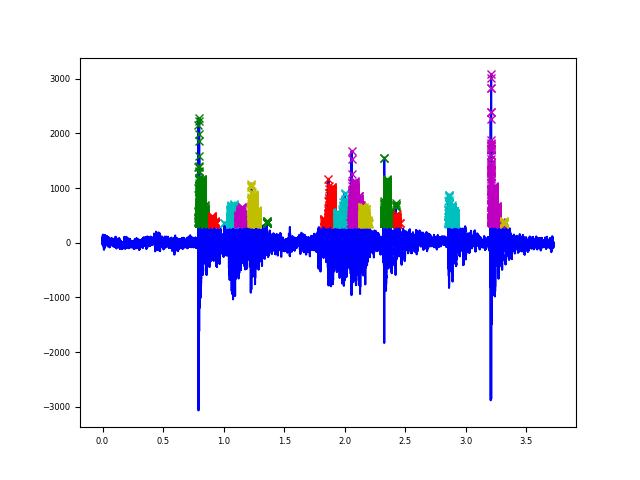
\includegraphics[width=0.8\textwidth]{Images/AcCAPPCHA/hello35_time}
     \caption{\footnotesize{Audio during insertion of password \texttt{hello35} all sub-windows highlighted.}}\label{AcCAPPCHA:hello35_time}
\end{figure}
\subsection{Character correspondence}\label{AcCAPPCHA:char_correspondence}
The character correspondence also looks for audio peaks during the insertion of the password. The identification of the peaks is performed by using also two threads as mentioned in time correspondence (see \myref{Character}{AcCAPPCHA:char_correspondence}). The thresholding parameters are obtained in the same way, by exploiting the noise peak, but character correspondence also analyses the shape of the audio signal recorded during the insertion of the password.\\
When a key is pressed by a user on the keyboard, it produces a variation of the audio signal, called \textit{press peak}, for a time window of about 8-10 ms\cite{keyboard_acoustic}. This signal shape in each window can also be divided in three consecutive and meaningful areas:
\begin{itemize}
\descItem{touch peak}{peak in a window of 2-3 ms, caused by the user's finger touching the key}
\item{\textbf{noisy meaningless area}}
\descItem{hit peak}{peak in a window of 2-3 ms at the end of 8-10 ms windows, caused by the finger and the key hitting the keyboard supporting plate.}
\end{itemize}
The first goal of character correspondence is to obtain the character related to each key pressed by the user. AcCAPPCHA extract information from the touch peak, that is the most significant, and the hit peak.\\
Following the idea of Asonov and Agrawal, I exploit deep learning to classify each pressed key. In the following sections, there is a detailed explanation of the main phases required and implemented for this classification method:
\begin{itemize}
\item{Data acquisition}
\item{Extraction of features}
\item{Neural network}
\item{Verification}
\end{itemize}
The first three phases were performed only once and it's not performed by the CAPTCHA. At the contrary the last step is performed at every insertion of the password by AcCAPPCHA.
In the first one I record audio files of every key press. From this audio files, I extract information from the peaks in the second phase and then I train a neural network using them in the third step. Hence the verification procedure is based only on: the detection of the audio peaks during the insertion of the password, the extraction of the information from every audio peaks and the classification of them through neural network trained at the previous steps.

\subsubsection{Data acquisition}
The dataset acquisition was performed using two tasks running in parallel: the first one is a key-logger that is used to organize all the recorded audio files in several directories and the second one that records an audio file for each key typed. The communication between the two threads is performed through the private members of the class, in which the thread are created, and the use of the mutual exclusion (mutex). The keylogger continues the acquisition of the audio files even if a special key is pressed (for example F3 button).\\
The choice of running two tasks in parallel is because the recording session must start before the key press and it must end a little bit later the acquisition of the character. In this way the shape of the signal of the audio peak, related to the key press, are not going to be cut. The data acquisition program can also acquire audio files for a series of key presses but in this case I decided to record one audio file for each key press.\\
In details the key-logger waits for the insertion of a single key by the user and then reports it to the thread that performs audio recording. This last task closes the audio stream and stores the audio signal into a \textit{wav} file named with a progressive number. All the audio files are dynamically organized into a set of subfolders of an output directory, each one with the name of the respective typed key.\\
The recording phase was performed using the built-in Realtek microphone and the keyboard of my MSI GL63 8RD laptop. The names of the subfolders (labels), in which each audio file of a press is inserted, are reported in \myref{Appendix}{chapter:KeyMapping}.\\
Looking at the Table in the Appendix, the keylogger  is evident. It maps each key to an ASCII string of upper or lower alphabetic characters because otherwise many keys would be mapped into invalid names of folders (for example, the key \textit{'.'} is now mapped into the label \textit{'POINT'}). Another observation about the table in \myref{Appendix}{chapter:KeyMapping} is that there are two columns of labels: the first one related to the label seen by the key-logger, the second one related to the label manually assigned by me to each key. Sometimes these labels differ for the same entry because of:
\begin{itemize}
\descItem{higher accuracy for spatial distribution of the keys on the keyboard}{for example, \textit{'INSERT'} and \textbf{'0\_INSERT'} (with Num lock on) would be mapped into \textit{'INSERT'} by the keylogger but they are considered different thanks to my map;}
\descItem{improvement of the the classification of the keys made by the keylogger}{for example, \textit{'ALT'} label is wrongly mapped into \textit{'SHIFT'} by the keylogger.}
\descItem{addition of keys mapped only on the hardware level}{\textit{FN} is the only key with this problem. The keylogger doesn't detect any key, when \textit{FN} is typed by the user. Hence I had to type \textit{FN}, followed by another key \textit{'a'}, so the audio files will be stored in \textit{'a'} subfolder. Then I rename the subfolder \textit{'FN'} and I create a python script to resize all the audio signals inside it and remove the useless second peak, related to \textit{'a'} press.}
\end{itemize}
The last two reasons are very important because they highlight also the power of acoustic side-channel. If an attacker implements an high-level keylogger exploiting also microphone information and remapping wrong labels, the accuracy of its software can increase very much with respect to a traditional keylogger without audio analysis. In fact the hacker could collect a dataset of recordings of pressed keys on the same type of the victim's keyboard and then it could train a Neural Network to use with malicious purposes.\\
However I record 200 audio signals for each key of my keyboard obtaining a dataset of 20400 audio files. I performed also Data Augmentation on them trying to improve the accuracy of the prediction for the neural network, using two approaches: 
\begin{itemize}
\descItem{Time-shift}{from each audio signal I created four new audio signals obtained by applying a time-shift respectively of 0.5, 1.0, 1.5 and 2.0 seconds.}
\descItem{Introduction of Gaussian noise}{from each audio signal I created four new audio signals by adding a sequence of random samples, taken from a Gaussian distribution with the standard deviation equal to 150 and the mean equal 0.}
\end{itemize}
Using these approaches I obtained a training set of 1800 audio signals for key, composed respectively by the following datasets:
\begin{itemize}
\item{200 audio signals manually recorded by me}
\item{800 audio signals obtained by time-shift technique}
\item{800 audio signals from introduction of Gaussian noise}
\end{itemize}
The accuracy of the Neural Network trained on audio signals of both first and second datasets is higher than the one related to the Network trained on first dataset only. The efficiency of the Neural Network trained on first and third dataset is worst than the one related to the network trained on only the first dataset.\\
I notice that the reason of the previous observation is that the third dataset has many signals, related to different keys, with FFT coefficients similar one to the other. Hence I used only the network trained on the first dataset and both on the first at the second dataset as prediction model. Considering that my keyboard is composed by 102 keys, I used respectively a dataset of 20400 and 102000 audio files to train the neural network.

\subsubsection{Classification}\label{AcCAPPCHA:classification}
During the classification phase, I decided how to extract the features from each audio peak, that will be used as input of a neural network. Then I use the features extracted from the audio files in the dataset to train my neural network. used to three different approaches, the first two \\
I tried three different approaches for the extraction of the features and for each them, the feature for each key is respectively composed by:
\begin{itemize}
\item{FFT coefficients of the touch peak}
\item{FFT coefficients of the hit peak and the touch peak}
\item{Features obtained from the hit peak and the touch peak using a deep learning pre-trained model}
\end{itemize}
The first two approaches come from the idea in the work of Asonov and Agrawal and the last one was based on the modern sound classification techniques. In the first two cases, the coefficients are extracted from a window of 3 ms around the peaks and then they are normalized in floating point values in range $[0, 1]$ (see \myref{Figure}{AcCAPPCHA:feature_example}).\\
In the third case, the touch peak and the hit peak samples, taken by 3ms windows, are concatenated and then the spectrogram is computed over these samples (see \myref{Figure}{AcCAPPCHA:spectrogram}). From the spectrogram, I extract a feature composed by 512 values through the use of the VGG16 convolutional neural network.\\
The network was pre-trained on the images in the \href{http://www.image-net.org/}{ImageNet} database and I used the intermediate results of neurons, before the last fully connected layers, as feature. The reason of this approach is that a pre-trained network already extracts very well features for good classification of a many labels and it can extract features better than a Convolutional Neural Network for image classification created from scratch.\\
The features obtained from the audio files are divide into three new dataset: the training set and the test set. \\
After the extraction of the features with the previous methods, I created a deep neural network from scratch. Its number of input neurons is equal to the size of a feature and the number of output neurons is equal to the number of keys to be mapped. I tried to insert several hidden layers composed by different number of neurons but after changing many parameters, I decided to use only one hidden layer 1024 neurons if the feature was obtained using the spectrograms and 100 otherwise. This choice comes from the best trade-off between the accuracy of the network on the test set and the prediction of labels for new audio peaks obtained later during the insertion of the password.
\begin{figure}[H]
     \centering
     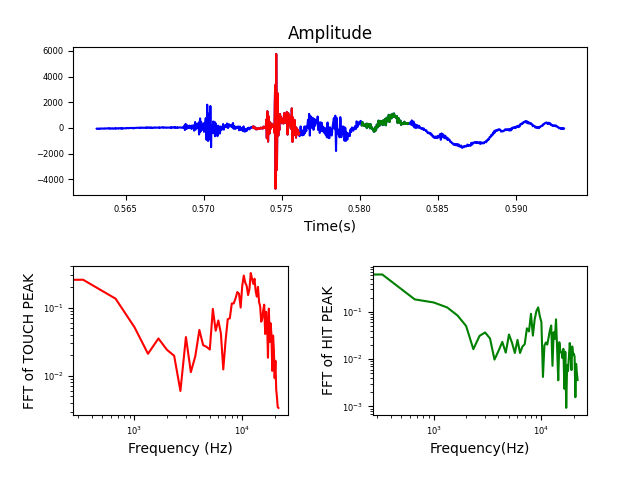
\includegraphics[width=.9\linewidth]{Images/AcCAPPCHA/feature_example}
     \caption{\footnotesize{Example of normalized FFT computation of the touch peak and the hit peak for an audio file of key \textit{'0'}.}}\label{AcCAPPCHA:feature_example}
\end{figure}
\begin{figure}[H]
     \centering
     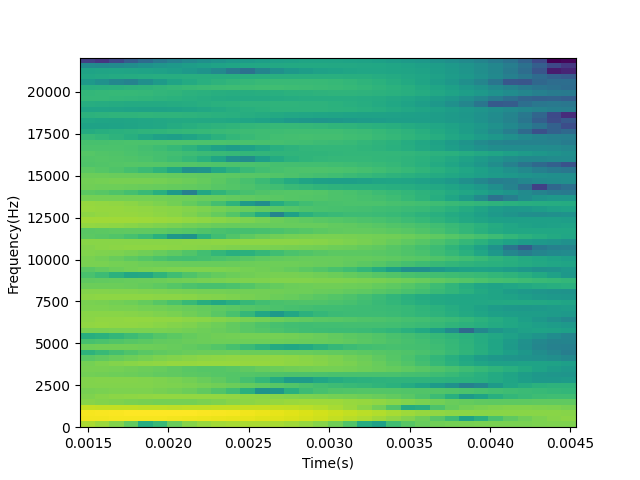
\includegraphics[width=.8\linewidth]{Images/AcCAPPCHA/spectrogram}
     \caption{\footnotesize{Example of spectrogram for an audio file of key \textit{'0'}.}}\label{AcCAPPCHA:spectrogram}
\end{figure}

\subsubsection{Verification}
The verification phase is performed by AcCAPPCHA. The audio signal, taken during the insertion of the password, is analysed and then the verification can be based on:
\begin{itemize}
\item{every audio peak obtained using threshold obtained from the noise evaluation}
\item{audio peaks related to the time instants of to the time correspondence}
\end{itemize}
After the selection of the previous peaks, AcCAPPCHA selects the touch and the hit peaks and it computes the features with the approach previously selected by the user from the ones reported in \myref{Section}{AcCAPPCHA:classification}. 


I perform the prediction using the Neural Network. I collect the most probable predicted keys and I repeat the procedure for every window initially computed on the audio. This method is very weak because after this phase, the algorithm tries to find an ordered sequence of characters, one from each window, that corresponds with the password inserted by the user. If this exists, AcCAPPCHA declares that the user was a human, otherwise a bot. The main problem of this approach is that there is no correspondence in time between a character belonging to the final sequence and the moment in which the same character was inserted physically by the user. In fact there can be false positives caused by the prediction from peak that are not related to the absolute maximum one. In other terms, in the set of the maximuma of all the windows there can be someone that is not related to the touch peak but to a local maximum.\\
The second approach solves the previous problem because the windows, where the maxima are looked for, are obtained by the correspondence time approach. In this case, AcCAPPCHA verification becomes more accurate in theory even if in practice the deep learning technique is not very efficient in prediction for a single key.

\section{Communication between client and server}
In the second phase, the username and the password of the user will be signed through ECDSA and sent by client to the authentication service if and only if the insertion was performed by a human. The algorithm that perform the evaluation of user activity (see \myref{Section}{AcCAPPCHA:user_activity}) is performed at client side but the value returned by it is evaluated at server-side. The response of the evaluation of user activity concatenated with a nonce and then signed through ECDSA, is sent to the server (see \myref{Section}{inv:communication}). The use of the nonce, unique and random generated sequence, is very important to guarantee that no reply attacks would be performed. In fact the server, after the reception of a message from the client, the server can check if the client has already sent the same nonce before and in this case it declines the message of the client. In this way, any attacker can't reuse a message that previously establishes a client was human. This type of procedure can be also useful to sign HTTP data, for example data sent using POST request (as insertion of password during authentication phase). In the testing phase I performed, I designed and implemented also a simplified version of the communication between the client and the server for an authentication service.\\
The application was tested on local network and the actions performed by involved parties are described in details in the following sections (see Figure ).
\begin{figure}
\centering
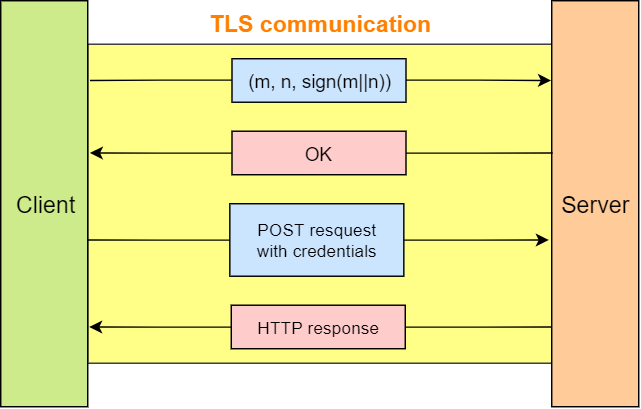
\includegraphics[width=.8\textwidth]{Images/AcCAPPCHA/client-server}
\end{figure}
\subsection{Client}
The client performs the authentication following these steps:
\begin{enumerate}
\item{It establishes a connection with the server over TLS layer to increase the security strength of the communication between the parties;}
\item{It sends the message $(m, n, sign(m||n))$ where:
\begin{itemize}
\item{$m$ is the string with the response of AcCAPPCHA algorithm on client side (\textit{'True'} if Human, \textit{False} if bot)}
\item{$n$ is the the nonce}
\item{$sign(m||n)$ is the ECDSA signature of the concatenation $m||n$ of the response and the nonce. For ECDSA was used SHA256 algorithm.}
\end{itemize}
From a practical point of view, I format the message in the following way:
\begin{table}[H]
\centering\footnotesize
\begin{tabular}{|c|}
\hline
\texttt{m CRLF n sign(m||n)}\\
\hline
\end{tabular}
\end{table}
According to basic rules in grammar of \textbf{HTTP/1.1} (see Section 2.2 of \href{https://tools.ietf.org/html/rfc2616}{RFC 2616}), \textit{CR} is the carriage return ('$\setminus r$') and LF is the line feed ('$\setminus n$'). The spaces in the message aren't considered. In this way, I can separate easily m looking at '$\setminus r\setminus n$'. The nonce has a fixed length of 16 bytes.}
\item{The client waits for response of the server with format:
\begin{table}[H]
\centering\footnotesize
\begin{tabular}{|c|}
\hline
\texttt{response CRLF}\\
\hline
\end{tabular}
\end{table}
If the answer is equal '$OK\setminus r\setminus n$', AcCAPPCHA will go on with the authentication step, otherwise the client-side application performs again the verification, asking again to user to insert the password. The maximum number of trials for a particular user is 3.}
\item{If everything goes well in the previous step, The client sends the credentials (username, password) to the server through a HTTP POST request to '/cgi-bin/auth' resource. The name of folder '/cgi-bin' comes from the standard name of the folder with functions and \textit{auth} is the name of the function that server will call. This naming approach was used very much in the past to separate functions code from pure HTML code. The password is not sent directly but it's hashed before using SHA512. The POST request used by the client has the following format:\\
\begin{table}[H]
\hspace{2cm}\centering\footnotesize
\begin{tabular}{|l|}
\hline
\texttt{POST /cgi-bin/auth HTTP/1.1} $\mathtt{\setminus r\setminus n}$\\
\texttt{Host: SP foo.example CRLF}\\
\texttt{Content-Type: SP application/x-www-form-urlencoded CRLF}\\
\texttt{Content-Length: SP SIZE CRLF CRLF}\\
\texttt{user = USERNAME $\mathtt{\&}$ pwd = HASHEDPWD}\\
\hline
\end{tabular}
\end{table}
where everything follows as before the grammar in \href{https://tools.ietf.org/html/rfc2616}{RFC 2616}). In fact also \textbf{SP} represents the space character as in the documentation. \textbf{SIZE}, \textbf{USERNAME} and \textbf{HASHEDPWD} are replaced respectively with the size of the HTTP body, the username of the client and its password hashed with SHA512.
}
\item{The client waits for the HTTP response of the server, containing HTML code as body. Then the client saves the code on the file system and opens the default web browser only to show. The HTML code is intended to show 3 possible scenarios: the user was correctly logged in, the user inserted wrong password, the username wasn't already stored on the server database.}
\end{enumerate}

\subsection{Server}
The client performs the authentication following these steps:
\begin{enumerate}
\item{It establishes a connection with the client, after his request, over TLS layer to increase the security strength of the communication between the parties;}
\item{It receives the message $(m, n, sign(m||n))$ and check the integrity of the message. To do it, the server decrypts the ECDSA signature using the client's ECDSA public key and compares the result with \textit{m||n}.}
\item{If compared messages were the same, the server checks if the nonce was already used by the same client. If so, the server thinks that there was an attacker that is performing a replay attack. If the nonce wasn't already used by the client, it will be stored in a dictionary to monitor clients activity. Each entry of the dictionary is composed by:
\begin{itemize}
\descItem{Key: IP address}{It is the IP address of the client and it is a simplification of the information that identifies a client. For example the client could be associated also to port number used to make the request, the Operating System on which the AcCAPPCHA was running on client-side or other useful parameters.}
\descItem{Value: list of nonces}{Every time a client performs a new verification request on the server, the nonce is added to the list related to its IP address in the dictionary.}
\end{itemize}
}
\item{If the nonce was used for the first time by the client, the server checks the value of the response received by the client. If the response is 'True', the server replies '$OK\setminus r\setminus n$' otherwise '$NO\setminus r\setminus n$'. If some error occurs it sends '$ERROR\setminus r\setminus n$' to the client. In the last two cases, the server terminates.}
\item{If the server doesn't terminate, it waits for the POST request from the client and analyses it to perform authentication service. The server replies to client with several status codes:
\begin{itemize}
\item{\textbf{501 (}Not implemented\textbf{)}\\
If the request is not a POST (e.g. GET)}
\item{\textbf{400 (}Bad Request\textbf{)}\\
If the number of the parameters in the POST body is different from 2 (username and password).}
\item{\textbf{200 (}OK\textbf{)}\\
If the number of the parameters in the POST body is equal to 2, the server will reply with an HTTP response with a body content depending on several cases:
\begin{itemize}
\descItem{User not in the database}{the server sends the following HTML code if the specified username isn't already stored in the database.
\begin{table}[H]
\hspace{2cm}\centering\footnotesize
\begin{tabular}{|p{6cm}|p{0.5cm}c}
\cline{1-1}
\texttt{\key{<!DOCTYPE html>}}&\multirow{7}{*}{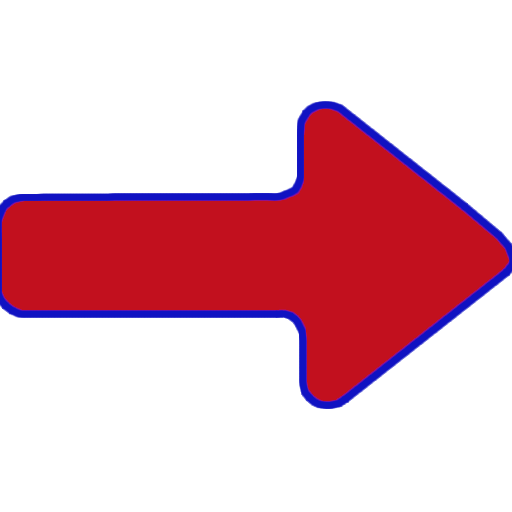
\includegraphics[width=0.5cm]{Images/arrow}}&\multirow{7}{*}{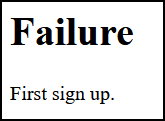
\includegraphics[scale=0.8]{Images/AcCAPPCHA/no_db_html}}\\
\texttt{\key{<html>}}&&\\
\texttt{\hspace{0.5cm}\key{<body>}}&\\
\texttt{\hspace{1.0cm}\key{<h1>}Failure\key{</h1>}}&&\\
\texttt{\hspace{1.0cm}\key{<p>}First sign up.\key{</p>}}&&\\
\texttt{\hspace{0.5cm}\key{</body>}}&&\\
\texttt{\key{</html>}}&&\\
\cline{1-1}
\end{tabular}
\end{table}
}
\descItem{Wrong password}{the server sends the following HTML code if the hashed password received from the client isn't the same with respect to the one stored in database for the specified username.
\begin{table}[H]
\hspace{2cm}\centering\footnotesize
\begin{tabular}{|p{6cm}|p{0.5cm}c}
\cline{1-1}
\texttt{\key{<!DOCTYPE html>}}&\multirow{7}{*}{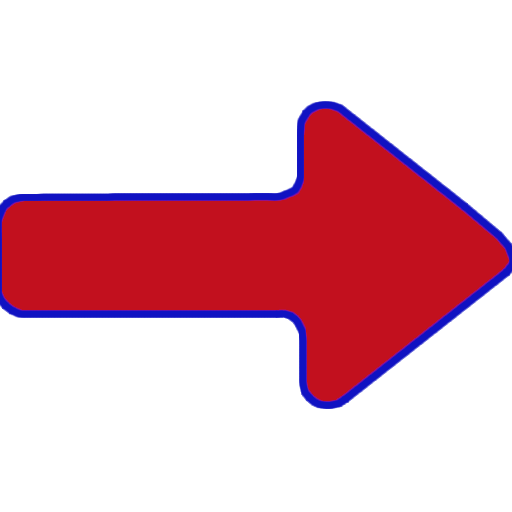
\includegraphics[width=0.5cm]{Images/arrow}}&\multirow{7}{*}{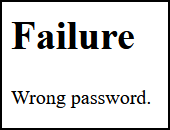
\includegraphics[scale=0.8]{Images/AcCAPPCHA/failure_html}}\\
\texttt{\key{<html>}}&&\\
\texttt{\hspace{0.5cm}\key{<body>}}&&\\
\texttt{\hspace{1.0cm}\key{<h1>}Failure\key{</h1>}}&&\\
\texttt{\hspace{1.0cm}\key{<p>}Wrong password.\key{</p>}}&&\\
\texttt{\hspace{0.5cm}\key{</body>}}&&\\
\texttt{\key{</html>}}&&\\
\cline{1-1}
\end{tabular}
\end{table}
}
\descItem{User logged in}{the server sends the following HTML code if the specified username exists in the database and  its hashed password stored in the database is the same of the one received through POST request.
\begin{table}[h]
\hspace{2.5cm}\centering\footnotesize
\begin{tabular}{|p{6cm}|p{0.5cm}c}
\cline{1-1}
\texttt{\key{<!DOCTYPE html>}}&\multirow{7}{*}{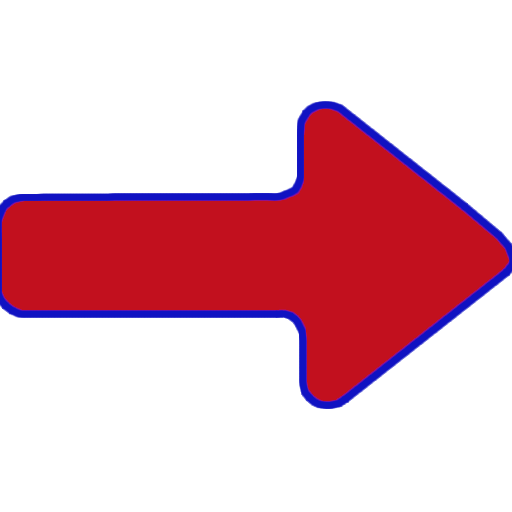
\includegraphics[width=0.5cm]{Images/arrow}}&\multirow{7}{*}{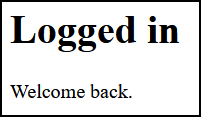
\includegraphics[scale=0.8]{Images/AcCAPPCHA/logged_html}}\\
\texttt{\key{<html>}}&&\\
\texttt{\hspace{0.5cm}\key{<body>}}&&\\
\texttt{\hspace{1.0cm}\key{<h1>}Logged in\key{</h1>}}&&\\
\texttt{\hspace{1.0cm}\key{<p>}Welcome back.\key{</p>}}&&\\
\texttt{\hspace{0.5cm}\key{</body>}}&&\\
\texttt{\key{</html>}}&&\\
\cline{1-1}
\end{tabular}
\end{table}
}
\end{itemize}
}
\end{itemize}
}
\end{enumerate}

\subsection{Database}
The database, created to simulate the search of a username by the server, was made using PostgreSQL. I could store all the information in a simple text file or a csv file but I decide to use this approach to be more flexible to future integration to more complex database.\\
The database is composed by only a table \texttt{CloudUser} to store information about user identity usually stored during the sign up phase. The creation of the database was performed through the following instructions:
\lstset{basicstyle=\footnotesize,breaklines=true}
\lstinputlisting[language=SQL]{../Code/PC/dat/db/db_creation.sql}
I created several domain to manage format of some information of the user. For example the password is a string of 128 characters because each password is hashed using SHA512 and then formatting the result as a string of hexadecimal values.
Then I populated the dataset with some entries, related to fake user, only for testing purpose. An example of inserted users is the following one:
\vspace{0.5cm}
\begin{lstlisting}[language=SQL, showstringspaces=false]
INSERT INTO CloudUser (Name,
                       Surname,
                       Username,
                       Email,
                       Sex,
                       Password)
                       
VALUES ('Raffaele', 
        'Di Nardo Di Maio', 
        'RaffaDNDM', 
        'example1@gmail.com', 
        'Male',
        HASHPASSWORD);
\end{lstlisting}
In practice, \texttt{HASHPASSWORD} is replaced by the string of 128 characters corresponding to the hashed password in hexadecimal format.

\subsection{Encryption Keys}
The creation of the TLS socket for the communication between the client and the server is done by using keys and certificates created thanks to the following bash instructions:
\vspace{0.3cm}
\begin{lstlisting}[language=bash, showstringspaces=false, tabsize=4]
openssl req -new -x509 -days 365 -nodes -out client.pem
		-keyout client.key
\end{lstlisting}
\begin{lstlisting}[language=bash, showstringspaces=false, tabsize=4]
openssl req -new -x509 -days 365 -nodes -out server.pem 
		-keyout server.key
\end{lstlisting}
OpenSSL is a open-source implementation of TLS/SSL protocols and, thanks to the option \texttt{-x509}, you can display certificates and also access to many signing protocols.
In particular, in the previous bash instructions, a X.509 Certificate Signing Request (CSR) is generated and signed for both the parties.\\
Thanks to \texttt{-nodes} the private key is created and not encrypted. The certificates are stored respectively in \textit{server.pem} for the server side and \textit{client.pem} for the client and they are valid for 365 days. The private keys are stored thanks to \texttt{-keyout} option in the \textit{client.pem} and \textit{server.key}.\\\\
The keys, used in ECDSA signing and verification, were created as follow from Python language instead of using a bash tool:
\vspace{0.3cm}
\begin{lstlisting}[language=python, showstringspaces=false, tabsize=4]
from ecdsa import *
from hashlib import sha256

PRIVATE_KEY = SigningKey.generate(curve=SECP256k1,
                                  hashfunc=sha256)

with open('ecdsa.key', 'w') as private_pem:
	private_pem.write(PRIVATE_KEY.to_pem().decode())

PUBLIC_KEY = PRIVATE_KEY.get_verifying_key()

with open('ecdsa.pem', 'w') as public_pem:
	public_pem.write(PUBLIC_KEY.to_pem().decode())
\end{lstlisting}
The \textit{ecdsa} module gives access to the management of operations performed by signing and verification phase. In this case the private key, used to sign a message from the client, was computed on the curve \texttt{SECP256k1} usually used in Bitcoin applications.